
\section{Introduction}
\begin{figure}[h]
 \centering
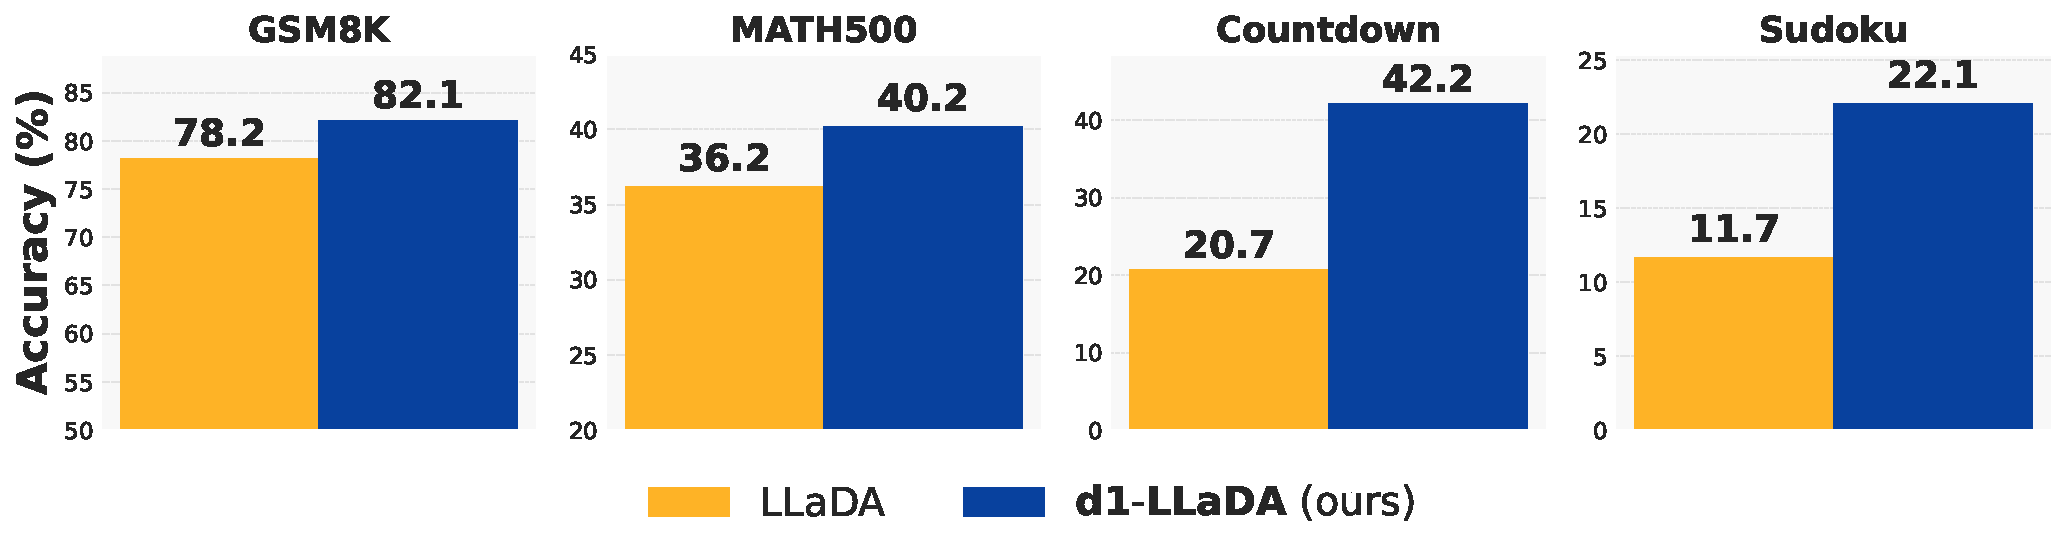
\includegraphics[width=\linewidth]{figs/separate_axes_chart.pdf}
 \caption{Across four math and planning tasks, \textbf{d1-LLaDA}, which undergoes SFT followed by our proposed \textbf{\grpo{}}, consistently outperforms the base LLaDA-8B-Instruct model. We report results using the best performing generation sequence length for each task and model, with complete sequence length results shown in \cref{tab:performance_results}.}
 
 \label{fig:pull}
\end{figure}



Recent advances in large language models (LLMs) have demonstrated remarkable capabilities across diverse applications spanning chatbots, coding, summarization, and translation~\citep{achiam2023gpt,dubey2024llama3herdmodels}. While these models typically scale through next-token prediction on vast corpora via computationally intensive pretraining, the finite availability of high-quality training data poses a fundamental scaling challenge. Reinforcement learning (RL) methods have emerged as a promising post-training method, enabling models to generate and explore with reward signals rather than relying solely on static datasets. This approach has yielded significant improvements on reasoning tasks in recent models, such as DeepSeek-R1~\citep{guo2025deepseek} and Kimi K1.5~\citep{team2025kimi},  demonstrating that applying RL directly to base models can achieve performance comparable to OpenAI's o1 model~\citep{o1}. However, these advances in RL-based post-training have primarily been limited to autoregressive LLMs that operate through left-to-right, sequential inference.


In a parallel line of work, discrete diffusion large language models (dLLMs) \citep{nie2025largelanguagediffusionmodels, gong2025scaling, nie2024scaling, dream2025} have emerged as promising non-autoregressive alternatives for language modeling. Unlike AR models that generate text token-by-token in a causal manner, dLLMs generate text through an iterative denoising process, refining sequences over multiple steps while leveraging both past and future context via bidirectional attention. Among them, open masked dLLMs such as LLaDA \citep{nie2025largelanguagediffusionmodels} have demonstrated performance comparable to similarly sized AR models, and closed-source dLLMs such as Mercury~\citep{inception2025mercury} further demonstrate excellent inference efficiency. However, leading open-source dLLMs have not undergone RL post-training, leaving this promising direction largely unexplored. This paradigm shift raises important questions about how RL post-training might be effectively realized in a non-autoregressive context.


Adapting RL algorithms to masked dLLMs poses  unique challenges because existing successful approaches for AR models, such as PPO~\citep{schulman2017proximal} and GRPO~\citep{shao2024deepseekmath}, rely on estimating and optimizing policy distributions through computing log-probabilities of generated sequences, which cannot be directly applied to dLLMs. While this computation is straightforward in AR models through sequential factorization, dLLMs lack this natural decomposition due to their iterative, non-sequential generation process.

To bridge this gap, \textbf{we propose d1, a two-stage post-training framework for enhancing reasoning in masked dLLMs}. In the first stage, the model undergoes supervised finetuning (SFT) on high-quality reasoning traces. \textbf{In the RL stage, we introduce \grpo{}}, a novel policy gradient method for masked dLLMs that builds upon GRPO with our proposed efficient one-step estimation of log-probabilities. To the best of our knowledge, this represents the first application of policy gradient RL to masked dLLMs. Our estimator leverages random prompt masking, which acts a form of regularization for policy optimization, allowing us to scale the number of gradient updates per batch and reduces the number of online generations required by RL training. This substantially reduces the compute time. 

Empirically, we instantiate d1 using LLaDA-8B-Instruct as our base model. We compare d1-LLaDA's performance with the base LLaDA model, as well as with LLaDA variants trained using SFT-only and \grpo-only approaches. Our experiments demonstrate that d1 consistently outperforms the base model across four reasoning tasks in math and planning, as shown in \cref{fig:pull}, with nearly doubled performance on planning tasks. Furthermore, d1 surpasses both the SFT-only and \grpo-only methods. Additionally, we complement our primary findings with thorough ablation studies on algorithm design, qualitative analysis, and extensions of \grpo{} to coding tasks, where we also observe consistent improvements.
